\documentclass[../Main.tex]{subfiles}
\usepackage{calc}
\usepackage{longtable}
\usepackage{tikz}
\usepackage{pgfplots}
\pgfplotsset{compat=1.18}
\usetikzlibrary{backgrounds}

\begin{document}
	\section{Proposed Research Model}
    This chapter introduces a comprehensive research model designed to examine the influence of university-based incubation programs (UBIs) on the performance of startups in Vietnam. The model posits that the core components of incubation support exert both direct and indirect effects on startup success, with the latter mediated by the development of a robust Entrepreneurial Orientation (EO) within the startup. The conceptual foundation of this model is rooted in the Resource-Based View (RBV), which underscores the significance of unique resources and capabilities in securing competitive advantage \autocite{barney1991firm}, and the Technology-Organization-Environment (TOE) framework, which highlights the interplay of technological, organizational, and environmental factors in shaping program outcomes.

    The proposed model, illustrating the relationships between the study's variables, is visually represented in the diagram below:
    \begin{figure}[H]
        \centering
        \includegraphics[width=\textwidth]{Figure/research_model.png}
        \caption{Proposed Research Model}
        \label{fig:research_model}
    \end{figure}

    The model is specifically tailored to Vietnam's developing entrepreneurial ecosystem, where startups face significant challenges such as limited funding, expertise, and market access. By examining the mediating role of EO, this research aims to provide a nuanced understanding of how UBIs create value, offering actionable insights for program optimization.

    \subsection{Literature Review of Key Factors}
    Table \ref{tab:literature_review_factors} presents a comprehensive overview of previous research examining the key factors in university-based incubation programs and their relationships with startup performance. This synthesis demonstrates the theoretical foundation and empirical evidence supporting the proposed research model.

    \begin{longtable}{|p{2.5cm}|p{3cm}|p{6cm}|p{2.5cm}|}
        \caption{Literature Review of Key Factors in University-Based Incubation}
        \label{tab:literature_review_factors} \\
        \hline
        \textbf{Factor} & \textbf{Key Studies} & \textbf{Main Findings} & \textbf{Context} \\
        \hline
        \endfirsthead
        \multicolumn{4}{c}%
        {\tablename\ \thetable\ -- \textit{Continued from previous page}} \\
        \hline
        \textbf{Factor} & \textbf{Key Studies} & \textbf{Main Findings} & \textbf{Context} \\
        \hline
        \endhead
        \hline \multicolumn{4}{r}{\textit{Continued on next page}} \\
        \endfoot
        \hline
        \endlastfoot
        
        \textbf{Mentorship Quality} & \autocite{jacobi1991mentorship} & Found that mentorship significantly enhances academic and professional development through knowledge transfer and confidence building & Educational \\
        & \autocite{ragins1999review} & Demonstrated that formal mentoring relationships lead to improved career outcomes and organizational performance & Organizational \\
        & \autocite{underhill2006mentoring} & Meta-analysis showing positive correlation between mentoring programs and workplace effectiveness & Workplace \\
        & \autocite{stjean2012mentoring} & Established direct link between mentoring quality and entrepreneurial success, particularly for novice entrepreneurs & Entrepreneurship \\
        & \autocite{sullivan2011effectiveness} & Found business development services, including mentoring, significantly improve SME performance in developing countries & Developing Markets \\
        \hline
        
        \textbf{Resource Access} & \autocite{barney1991firm} & Resource-Based View theory: access to valuable, rare, and inimitable resources creates competitive advantages & Theoretical \\
        & \autocite{mian1996assessing} & Demonstrated that access to university resources significantly enhances incubator tenant performance & University Incubators \\
        & \autocite{bruneel2010funding} & Found that funding access through university spin-offs improves venture performance and survival rates & University Spin-offs \\
        & \autocite{cooper1994initial} & Established that initial financial and human capital resources predict new venture performance & New Ventures \\
        & \autocite{bruton2010governance} & Showed that resource availability significantly influences startup strategic behavior in emerging markets & Emerging Markets \\
        \hline
        
        \textbf{Networking Opportunities} & \autocite{granovetter1973strength} & Social Network Theory: weak ties provide access to diverse information and opportunities & Theoretical \\
        & \autocite{stam2008entrepreneurial} & Found that network centrality and diversity positively influence entrepreneurial orientation and performance & Entrepreneurship \\
        & \autocite{batjargal2003social} & Longitudinal study showing social capital and network relationships enhance entrepreneurial performance in emerging markets & Emerging Markets \\
        & \autocite{theodorakopoulos2014business} & Identified networking as a key success factor in business incubation programs & Business Incubation \\
        & \autocite{harper2018makes} & Found that effective networking opportunities distinguish successful from unsuccessful incubators & Incubator Performance \\
        \hline
        
        \textbf{Entrepreneurial Orientation} & \autocite{miller1983correlates} & Established EO as a fundamental strategic orientation driving organizational performance & Strategic Management \\
        & \autocite{covin1989strategic} & Demonstrated that EO enables firms to adapt to changing environments and achieve superior performance & Strategic Management \\
        & \autocite{lumpkin1996clarifying} & Clarified EO construct and established its positive relationship with firm performance & Entrepreneurship \\
        & \autocite{rauch2009entrepreneurial} & Meta-analysis confirming positive relationship between EO and firm performance across various contexts & Meta-analysis \\
        & \autocite{saeed2014entrepreneurial} & Found EO particularly beneficial in emerging markets and dynamic environments & Emerging Markets \\
        & \autocite{wales2013entrepreneurial} & Demonstrated EO's multilevel impact on organizational performance & Multilevel Analysis \\
        \hline
        
        \textbf{Startup Performance} & \autocite{patton2014realising} & Comprehensive study of business incubation impact on startup performance metrics & Business Incubation \\
        & \autocite{barbero2012revisiting} & Comparative study showing performance differences between European and US incubators & International Comparison \\
        & \autocite{Chan2005Assessing} & Developed framework for assessing technology incubator program effectiveness & Technology Incubation \\
        & \autocite{spigel2017relational} & Found that relational aspects of entrepreneurial ecosystems significantly influence startup performance & Ecosystem Theory \\
        & \autocite{al2017challenges} & Identified key challenges and opportunities affecting incubator performance and outcomes & Incubator Challenges \\
        \hline
        
        \textbf{Innovation Performance} & \autocite{schumpeter1934theory} & Innovation Theory: entrepreneurial orientation drives innovative outcomes & Theoretical \\
        & \autocite{lumpkin1996clarifying} & Found innovativeness component of EO directly leads to new product and process development & Innovation \\
        & \autocite{wiklund2003knowledge} & Demonstrated that EO's innovativeness dimension positively associates with various innovation outcomes & Knowledge-based Resources \\
        \hline
        
        \textbf{Market Performance} & \autocite{narver1990effect} & Market Orientation Theory: proactive market strategies lead to superior market performance & Market Theory \\
        & \autocite{lieberman1988first} & First-Mover Advantage Theory: early market entry provides competitive advantages & Competitive Strategy \\
        & \autocite{lumpkin2001linking} & Found EO's proactiveness and risk-taking dimensions positively associate with market performance & Market Performance \\
        \hline
        
        \textbf{Financial Performance} & \autocite{porter1980competitive} & Strategic Management Theory: strategic orientations creating competitive advantages lead to superior financial performance & Strategic Management \\
        & \autocite{rauch2009entrepreneurial} & Meta-analysis showing EO positively associated with financial performance indicators & Financial Performance \\
        & \autocite{saeed2014entrepreneurial} & Found EO particularly beneficial for financial performance in emerging markets & Emerging Markets \\
        \hline
    \end{longtable}

    \section{Variables of the Study}
    The research model is constructed upon a carefully selected set of variables that collectively capture the multifaceted dynamics of university-based incubation in Vietnam. The dependent variable, startup performance, is conceptualized as a multidimensional construct encompassing innovative, market, and financial dimensions. This approach moves beyond traditional financial metrics, recognizing that the success of a new venture is reflected not only in revenue growth and profitability but also in its capacity for innovation and market expansion. The RBV framework supports this perspective by asserting that superior performance arises from the effective deployment of valuable resources and capabilities, while the TOE framework situates performance within the broader context of technological, organizational, and environmental influences.

    To ensure robust measurement, startup performance will be assessed using both quantitative and qualitative data. Objective indicators such as the number of new products launched, patents filed, market share growth, and revenue increases will be complemented by founders' subjective evaluations, captured through a Likert-scale survey. This mixed-methods approach is particularly relevant in the Vietnamese context, where startups often operate under resource constraints and face significant barriers to market entry.

    The independent variables in this study represent the principal forms of support provided by UBIs: mentorship quality, resource access, and networking opportunities. Mentorship quality refers to the caliber and effectiveness of guidance offered by mentors, encompassing strategic, technical, and operational advice. In Vietnam, where experienced business leaders are scarce, UBIs play a critical role by leveraging academic and industry expertise to support nascent ventures. Resource access includes both tangible assets, such as funding and infrastructure, and intangible resources, such as privileged access to university research facilities. Given the persistent challenges Vietnamese startups face in securing capital and technology, this variable is of particular importance. Networking opportunities capture the incubator's role in facilitating connections with investors, industry partners, and peer entrepreneurs, which are essential for overcoming the limitations of Vietnam's relatively underdeveloped entrepreneurial networks.

    Entrepreneurial Orientation (EO) serves as the mediating variable, reflecting a firm's strategic posture toward innovation, proactiveness, and risk-taking. EO is not merely an outcome but a dynamic capability that enables startups to leverage incubation support effectively. In the Vietnamese market, characterized by rapid change and intense competition, a strong EO is indispensable for survival and growth.

    To control for extraneous influences, the model incorporates several control variables, including startup age, industry sector, founder experience, and university type. These factors are included to account for variations in performance that may arise from differences in maturity, sectoral dynamics, managerial expertise, or institutional context.

    \section{Research Methodology}
    \label{section:4.2_Research_methodology}

    \subsection{Research Design}
    \label{subsection:4.2.1_Research_design}
    A sequential explanatory mixed-methods design is employed, starting with quantitative data collection and analysis to identify significant relationships, followed by qualitative data collection to explain and elaborate on these findings \autocite{creswell2014research}. This research adopts a mixed-methods approach combining systematic literature review with quantitative survey methodology. The design follows a sequential explanatory approach where literature review findings inform survey development. The research framework is grounded in the Resource-Based View (RBV) theory, examining how UBI resources contribute to startup performance through the mediating role of Entrepreneurial Orientation. The design ensures methodological rigor while maintaining practical relevance for Vietnam's entrepreneurial ecosystem.

    \begin{condensed_idea}[Research Design of the Thesis]
        This thesis will employ a sequential explanatory mixed-methods design, a \textbf{two-phase approach} to understand the impact of University Business Incubator (UBI) support on startup performance.
    
        \textbf{First phase:} This involves quantitative data collection and analysis. This measures Startup Performance, UBI-provided Resources, and UBI-facilitated Networks using both objective metrics (e.g., survival rates, funding, infrastructure access, investor introductions) and perceptual Likert scale surveys. The goal is to identify broad relationships and trends.
    
        \textbf{Second phase:} This utilizes qualitative data collection and analysis through the archival study of publicly available online resources. This qualitative data serves to explain and elaborate on the initial quantitative findings, particularly focusing on the nuanced ways in which resources and networks interact and are utilized by founders to enhance startup success.
    \end{condensed_idea}

    \subsection{Key Constructs and Operationalization}
    The operationalization of key constructs in this study follows established methodological frameworks in entrepreneurship research. Startup Performance serves as the dependent variable, measured through a multi-faceted approach that captures various dimensions of success. Quantitative measures include survival rate, revenue growth, funding raised, job creation, and intellectual property generated, with data collected from UBI records and public databases such as Crunchbase. Perceptual measures encompass self-reported perceived success by founders regarding achievement of milestones and market penetration, utilizing Likert scale surveys to capture subjective assessments of performance outcomes.

    Resources provided by UBIs, aligned with the Resource-Based View framework, capture the internal assets and support mechanisms available to incubated startups. Quantitative measures focus on access to physical infrastructure, training hours provided, seed funding amounts, and mentor-hours facilitated. Perceptual measures assess startup founders' evaluations of UBI-provided workspace quality, mentorship effectiveness, training program utility, and administrative support value, measured through Likert scales in surveys \autocite{mian1996assessing}. This dual approach ensures comprehensive assessment of both objective resource availability and subjective resource utilization.

    Networks facilitated by UBIs, drawing from Entrepreneurial Ecosystem Theory, assess the external connections enabled through incubation programs. Quantitative measures include the number of investor introductions, strategic partnerships established, and successful collaborations with ecosystem actors such as corporations and research centers. Perceptual measures evaluate founders' assessments of UBI effectiveness in connecting them to investors, industry experts, potential customers, and peer networks, measured through Likert scales \autocite{theodorakopoulos2014business, harper2018makes}. The interaction construct, crucial to the proposed integrated model, assesses how resources and networks mutually enhance each other through survey questions designed to capture the extent to which network connections facilitate resource utilization and amplify training impact.

    \subsection{Data Collection}
    \label{subsection:4.2.2_Data_collection}
    The data collection process involves two primary methods: systematic literature review and quantitative survey. The systematic literature review utilizes academic databases including Google Scholar, ResearchGate, and ScienceDirect, with articles screened based on peer-reviewed status, publication between 2012 and 2025, and direct relevance to UBIs and startup performance. The quantitative survey targets at least 90 startup founders or managers associated with UBIs in Vietnam, using non-probability sampling methods. Survey distribution occurs via email and in-person at UBI-related events to ensure high response quality and representativeness.

    The target population encompasses current and alumni startups from a representative sample of UBIs, with preference for a longitudinal approach tracking startup cohorts over several years where feasible. Quantitative data collection employs online surveys administered to founders of UBI-incubated startups, including both current participants and alumni. These structured questionnaires incorporate sections on UBI resource perception, network effectiveness, and self-reported performance metrics, with anonymity ensured to encourage candid responses. Archival data collection supplements survey responses through official records from participating UBIs regarding services provided, funding history of incubated companies, graduation rates, and other verifiable performance metrics. This approach is complemented by data from publicly available sources including company websites, financial news, and startup databases, following methodologies similar to those used in large-scale incubator evaluations \autocite{patton2014realising}.

    Qualitative data collection utilizes archival internet research to complement quantitative findings through systematic review of materials related to surveyed startups and their respective UBIs. Sources include company websites, press releases, news articles, blog posts from founders or key personnel, and professional networking profiles such as LinkedIn. This archival approach provides rich, contextual narratives that elaborate on the underlying mechanisms behind statistical relationships identified in the quantitative phase, offering deeper insights into the complex interactions between resources and networks in startup development.

    \subsection{Data Analysis}
    \label{subsection:4.2.3_Data_analysis}
    Data analysis employs both qualitative and quantitative approaches to ensure comprehensive understanding of UBI impact on startup performance. Literature review findings are categorized thematically to identify UBI success factors and theoretical frameworks, while survey responses undergo statistical analysis including regression analysis to quantify the effects of UBI factors on startup performance and test the mediating role of Entrepreneurial Orientation. The analysis incorporates both descriptive statistics and inferential statistical techniques to ensure robust findings.

    Quantitative data analysis begins with descriptive statistics to summarize all variables, providing overview of means, standard deviations, and frequencies across the dataset. Multiple linear regression analysis examines direct relationships between Resources, Networks, and Startup Performance, with interaction terms included in regression models to test synergistic effects proposed by the integrated model \autocite{al2017challenges}. Control variables such as startup age, industry sector, founder experience, and initial capital are incorporated into regression models to mitigate confounding effects and ensure accurate estimation of UBI impact.

    Qualitative data analysis utilizes thematic analysis of collected online sources, with text-based data coded to identify recurring themes and patterns related to resource utility, network impact, and perceived interaction between these elements. This approach helps explain and elaborate on quantitative findings, particularly regarding the complex interaction variable. Selected case studies constructed from archival data highlight different ways resources and networks contribute to performance, demonstrating how their interaction manifests in real-world scenarios. The integration of quantitative and qualitative findings provides comprehensive understanding of both statistical relationships and underlying mechanisms, offering deeper insights into the complex dynamics of UBI support systems.

    \subsection{Ethical Considerations}
    Ethical considerations are rigorously observed throughout the study to ensure research integrity and participant protection. For quantitative surveys, informed consent is obtained from all participants, with clear communication regarding research purpose, voluntary participation nature, and withdrawal rights. All survey data undergoes anonymization and secure storage to ensure confidentiality. The qualitative component, relying on publicly available internet sources, focuses on organizational information in the public domain while minimizing personal data usage. When referencing specific cases, information is presented in ways that respect professional integrity and maintain ethical standards throughout the research process.

    This comprehensive methodology provides robust evidence for the proposed integrated model, offering valuable insights into how UBIs can strategically optimize their resource provision and network facilitation to maximize startup performance within broader entrepreneurial ecosystems.

    \section{Hypothesis Development}
    The following hypotheses are formulated to empirically test the relationships proposed in the research model. Each hypothesis is grounded in established theoretical frameworks and supported by empirical evidence, ensuring a rigorous approach to understanding the dynamics of university-based incubation in Vietnam.

    \subsection{Hypothesis Overview and Theoretical Framework}
    Table \ref{tab:hypothesis_summary} provides a comprehensive overview of all ten hypotheses, their theoretical foundations, expected relationships, and empirical support. This systematic approach ensures that each hypothesis is theoretically grounded and empirically testable.

    \begin{table}[H]
        \centering
        \caption{Summary of Research Hypotheses and Theoretical Foundations}
        \label{tab:hypothesis_summary}
        \begin{longtable}{|p{1.5cm}|p{3cm}|p{4cm}|p{3cm}|p{2.5cm}|}
            \hline
            \textbf{Hypothesis} & \textbf{Relationship} & \textbf{Theoretical Foundation} & \textbf{Expected Impact} & \textbf{Empirical Support} \\
            \hline
            \endfirsthead
            \multicolumn{5}{c}%
            {\tablename\ \thetable\ -- \textit{Continued from previous page}} \\
            \hline
            \textbf{Hypothesis} & \textbf{Relationship} & \textbf{Theoretical Foundation} & \textbf{Expected Impact} & \textbf{Empirical Support} \\
            \hline
            \endhead
            \hline \multicolumn{5}{r}{\textit{Continued on next page}} \\
            \endfoot
            \hline
            \endlastfoot
            
            \textbf{H1} & Mentorship Quality to EO & RBV, Social Learning Theory & Enhanced strategic orientation & \autocite{bandura1997self, zhao2005developing} \\
            \hline
            \textbf{H2} & Resource Access to EO & RBV, Resource Dependency Theory & Stronger innovative/proactive stance & \autocite{wiklund2005entrepreneurial, bruton2010governance} \\
            \hline
            \textbf{H3} & Networking to EO & Social Network Theory, RBV & Improved strategic positioning & \autocite{stam2008entrepreneurial, batjargal2003social} \\
            \hline
            \textbf{H4} & EO to Startup Performance & Strategic Management, Dynamic Capabilities & Superior overall performance & \autocite{rauch2009entrepreneurial, saeed2014entrepreneurial} \\
            \hline
            \textbf{H5} & EO to Innovation Performance & Innovation Theory, RBV & Enhanced innovation outcomes & \autocite{lumpkin1996clarifying, wiklund2003knowledge} \\
            \hline
            \textbf{H6} & EO to Market Performance & Market Orientation, First-Mover Advantage & Improved market position & \autocite{lumpkin2001linking, wiklund2005entrepreneurial} \\
            \hline
            \textbf{H7} & EO to Financial Performance & Strategic Management, RBV & Better financial returns & \autocite{rauch2009entrepreneurial, wales2013entrepreneurial} \\
            \hline
            \textbf{H8} & Mentorship Quality to Performance & Human Capital, Social Capital Theory & Direct performance improvement & \autocite{stjean2012mentoring, sullivan2011effectiveness} \\
            \hline
            \textbf{H9} & Resource Access to Performance & RBV, Resource Dependency Theory & Immediate operational benefits & \autocite{cooper1994initial, bruton2010governance} \\
            \hline
            \textbf{H10} & Networking to Performance & Social Network Theory, Social Capital Theory & Enhanced market access & \autocite{stam2008entrepreneurial, batjargal2003social} \\
            \hline
        \end{longtable}
    \end{table}

    \subsection{Theoretical Framework Integration}
    Figure \ref{fig:theoretical_framework} illustrates the integration of multiple theoretical perspectives that underpin the research hypotheses. This framework demonstrates how different theories complement each other in explaining the complex relationships between UBI support mechanisms and startup performance.

    \begin{figure}[H]
        \centering
        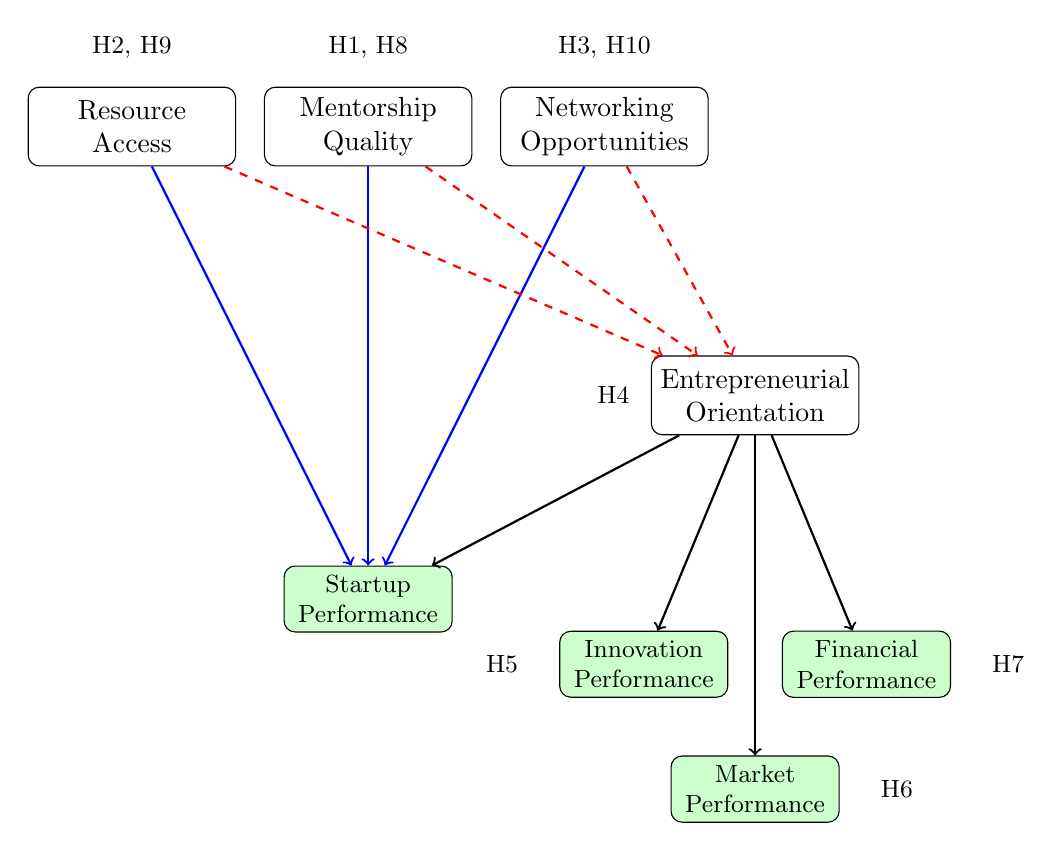
\begin{tikzpicture}[
            node distance=2cm,
            box/.style={rectangle, draw, rounded corners, minimum width=2.5cm, minimum height=1cm, text centered, text width=2.4cm},
            arrow/.style={->, thick},
            direct/.style={->, thick, blue},
            indirect/.style={->, thick, red, dashed},
            performance/.style={rectangle, draw, rounded corners, fill=green!20, minimum width=2cm, minimum height=0.8cm, text centered, text width=1.9cm, font=\small}
            ]
            
            % Independent variables
            \node[box] (mentorship) {Mentorship Quality};
            \node[box, left of=mentorship, xshift=-1cm] (resources) {Resource Access};
            \node[box, right of=mentorship, xshift=1cm] (networking) {Networking Opportunities};
            
            % Mediating variable
            \node[box, below right of=networking, yshift=-2cm, xshift=0.5cm] (eo) {Entrepreneurial Orientation};
            
            % Performance variables
            \node[performance, below of=mentorship, yshift=-4cm] (overall) {Startup Performance};
            \node[performance, below left of=eo, yshift=-2cm] (innovation) {Innovation Performance};
            \node[performance, below right of=eo, yshift=-2cm] (financial) {Financial Performance};
            \node[performance, below of=eo, yshift=-3cm] (market) {Market Performance};
            
            % Direct effects (H8-H10)
            \draw[direct] (mentorship) -- (overall);
            \draw[direct] (resources) -- (overall);
            \draw[direct] (networking) -- (overall);
            
            % Indirect effects through EO (H1-H3)
            \draw[indirect] (mentorship) -- (eo);
            \draw[indirect] (resources) -- (eo);
            \draw[indirect] (networking) -- (eo);
            
            % EO to performance (H4-H7)
            \draw[arrow] (eo) -- (overall);
            \draw[arrow] (eo) -- (innovation);
            \draw[arrow] (eo) -- (financial);
            \draw[arrow] (eo) -- (market);
            
            % Labels
            \node[above of=mentorship, yshift=-1cm] {\small H1, H8};
            \node[above of=resources, yshift=-1cm] {\small H2, H9};
            \node[above of=networking, yshift=-1cm] {\small H3, H10};
            \node[left of=eo, xshift=0.2cm] {\small H4};
            \node[left of=innovation, xshift=0.2cm] {\small H5};
            \node[right of=market, xshift=-0.2cm] {\small H6};
            \node[right of=financial, xshift=-0.2cm] {\small H7};
            
        \end{tikzpicture}
        \caption{Integrated Theoretical Framework Supporting Research Hypotheses}
        \label{fig:theoretical_framework}
    \end{figure}

    \subsection{Hypothesis 1 (H1): Mentorship Quality to Entrepreneurial Orientation}
    \textbf{H1: Mentorship quality is positively related to Entrepreneurial Orientation.}

    \subsubsection{Theoretical Foundation}
    \textbf{Resource-Based View (RBV)} \autocite{barney1991firm}: Access to valuable, rare, and inimitable resources creates competitive advantages. 
    \textbf{Social Learning Theory} \autocite{bandura1997self}: Entrepreneurs acquire strategic behaviors through observation and interaction with experienced mentors. 
    \textbf{Human Capital Theory} \autocite{becker1964human}: Knowledge and skills acquired through mentoring enhance entrepreneurial capabilities.

    \subsubsection{Mechanisms of Influence}
    Figure \ref{fig:h1_mechanisms} illustrates the key mechanisms through which mentorship quality enhances entrepreneurial orientation:

    \begin{figure}[H]
        \centering
        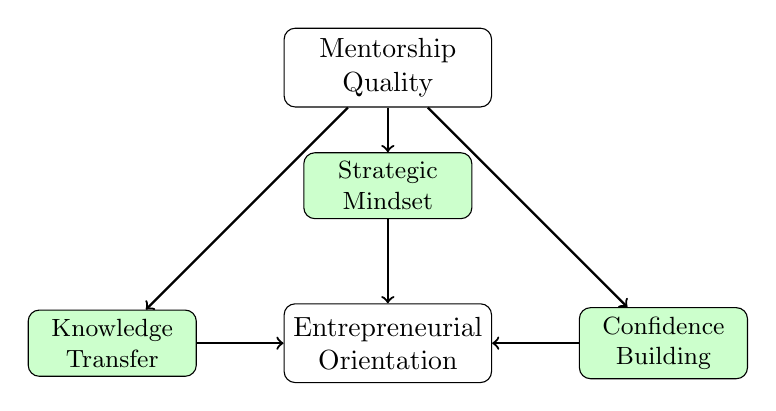
\begin{tikzpicture}[
            node distance=1.5cm,
            box/.style={rectangle, draw, rounded corners, minimum width=2.5cm, minimum height=1cm, text centered, text width=2.4cm},
            arrow/.style={->, thick},
            mechanism/.style={rectangle, draw, rounded corners, fill=green!20, minimum width=2cm, minimum height=0.8cm, text centered, text width=1.9cm, font=\small}
            ]
            
            % Main variables
            \node[box] (mentorship) {Mentorship Quality};
            \node[box, below of=mentorship, yshift=-2cm] (eo) {Entrepreneurial Orientation};
            
            % Mechanism boxes
            \node[mechanism, left of=eo, xshift=-2cm] (knowledge) {Knowledge Transfer};
            \node[mechanism, right of=eo, xshift=2cm] (confidence) {Confidence Building};
            \node[mechanism, above of=eo, yshift=0.5cm] (mindset) {Strategic Mindset};
            
            % Arrows
            \draw[arrow] (mentorship) -- (knowledge);
            \draw[arrow] (mentorship) -- (confidence);
            \draw[arrow] (mentorship) -- (mindset);
            \draw[arrow] (knowledge) -- (eo);
            \draw[arrow] (confidence) -- (eo);
            \draw[arrow] (mindset) -- (eo);
            
        \end{tikzpicture}
        \caption{Mechanisms Linking Mentorship Quality to Entrepreneurial Orientation}
        \label{fig:h1_mechanisms}
    \end{figure}

    \subsubsection{Contextual Relevance in Vietnam}
    In Vietnam's entrepreneurial ecosystem, mentorship quality is particularly critical due to several contextual factors:

    \textbf{Experience Gap}: Many young founders lack managerial and strategic experience. 
    \textbf{Educational Focus}: Traditional emphasis on technical skills over entrepreneurial thinking. 
    \textbf{Market Complexity}: Rapidly changing business environment requiring expert guidance. 
    \textbf{Network Limitations}: Limited access to experienced business leaders outside UBIs.

    \subsubsection{Empirical Evidence}
    Table \ref{tab:h1_evidence} summarizes key empirical studies supporting the relationship between mentorship quality and entrepreneurial orientation:

    \begin{table}[H]
        \centering
        \caption{Empirical Evidence for H1: Mentorship Quality to Entrepreneurial Orientation}
        \label{tab:h1_evidence}
        \begin{tabular}{|p{3cm}|p{4cm}|p{3cm}|p{2cm}|}
            \hline
            \textbf{Study} & \textbf{Key Finding} & \textbf{Context} & \textbf{Effect Size} \\
            \hline
            \autocite{bandura1997self} & Mentorship enhances entrepreneurial self-efficacy & General & Large \\
            \hline
            \autocite{zhao2005developing} & Mentoring mediates entrepreneurial intentions & Students & Medium \\
            \hline
            \autocite{stjean2012mentoring} & Direct link between mentoring and entrepreneurial success & Novice Entrepreneurs & Large \\
            \hline
            \autocite{sullivan2011effectiveness} & Business development services improve SME performance & Developing Countries & Medium \\
            \hline
        \end{tabular}
    \end{table}

    \subsection{Hypothesis 2 (H2): Resource access is positively related to Entrepreneurial Orientation}

    \subsubsection{Theoretical Foundation}
    This hypothesis draws upon several complementary theoretical perspectives:

    \begin{itemize}
        \item \textbf{Resource-Based View (RBV)} \autocite{barney1991firm}: Access to valuable, rare, and inimitable resources creates competitive advantages
        \item \textbf{Resource Dependency Theory} \autocite{pfeffer1978external}: Organizations' strategic behaviors are shaped by their access to critical resources
        \item \textbf{Resource Slack Theory} \autocite{cyert1963behavioral}: Having resources beyond immediate needs enables innovative and proactive strategies
    \end{itemize}

    \subsubsection{Types of Resources and Their Impact}
    Figure \ref{fig:h2_resources} categorizes the key resources provided by UBIs and their specific contributions to entrepreneurial orientation:

    \begin{figure}[H]
        \centering
        \begin{tikzpicture}[
            node distance=2.2cm,
            box/.style={rectangle, draw, rounded corners, minimum width=2.5cm, minimum height=1cm, text centered, text width=2.4cm},
            arrow/.style={->, thick},
            resource/.style={rectangle, draw, rounded corners, fill=orange!20, minimum width=2cm, minimum height=0.8cm, text centered, text width=1.9cm, font=\small},
            impact/.style={rectangle, draw, rounded corners, fill=red!20, minimum width=2cm, minimum height=0.8cm, text centered, text width=1.9cm, font=\small}
            ]
            
            % Main variable
            \node[box] (resources) {Resource Access};
            \node[box, below=5cm of resources] (eo) {Entrepreneurial Orientation};
            
            % Resource types
            \node[resource, left=3.5cm of resources] (financial) {Financial Resources};
            \node[resource, right=3.5cm of resources] (physical) {Physical Infrastructure};
            \node[resource, above=2cm of resources] (intellectual) {Intellectual Resources};
            \node[resource, below=2cm of resources] (human) {Human Resources};
            
            % Impact types
            \node[impact, left=3.5cm of eo] (innovative) {Innovativeness};
            \node[impact, right=3.5cm of eo] (proactive) {Proactiveness};
            \node[impact, below=2cm of resources] (risk) {Risk-taking};
            
            % Arrows for resources
            \draw[arrow] (financial) -- (resources);
            \draw[arrow] (physical) -- (resources);
            \draw[arrow] (intellectual) -- (resources);
            \draw[arrow] (human) -- (resources);
            
            % Arrows for impacts
            \draw[arrow] (resources) -- (innovative);
            \draw[arrow] (resources) -- (proactive);
            \draw[arrow] (resources) -- (risk);
            \draw[arrow] (innovative) -- (eo);
            \draw[arrow] (proactive) -- (eo);
            \draw[arrow] (risk) -- (eo);
            
        \end{tikzpicture}
        \caption{Resource Types and Their Impact on Entrepreneurial Orientation}
        \label{fig:h2_resources}
    \end{figure}

    \subsubsection{Vietnamese Context and Resource Challenges}
    The Vietnamese startup ecosystem faces specific resource constraints that make UBI support particularly valuable:

    \textbf{Capital Scarcity}: Limited access to venture capital and angel investment. 
    \textbf{Technology Gap}: Insufficient access to advanced technology and R\&D facilities. 
    \textbf{Infrastructure Limitations}: Inadequate office space and business support facilities. 
    \textbf{Expertise Shortage}: Limited availability of experienced business professionals.

    \subsubsection{Empirical Evidence}
    Table \ref{tab:h2_evidence} presents empirical studies demonstrating the relationship between resource access and entrepreneurial orientation:

    \begin{table}[H]
        \centering
        \caption{Empirical Evidence for H2: Resource Access to Entrepreneurial Orientation}
        \label{tab:h2_evidence}
        \begin{tabular}{|p{3cm}|p{4cm}|p{3cm}|p{2cm}|}
            \hline
            \textbf{Study} & \textbf{Key Finding} & \textbf{Context} & \textbf{Effect Size} \\
            \hline
            \autocite{wiklund2005entrepreneurial} & Resource availability positively associated with EO & SMEs & Large \\
            \hline
            \autocite{bruton2010governance} & Financial resources influence strategic behavior & Emerging Markets & Medium \\
            \hline
            \autocite{mian1996assessing} & University resources enhance incubator tenant performance & University Incubators & Large \\
            \hline
            \autocite{cooper1994initial} & Initial resources predict new venture performance & New Ventures & Large \\
            \hline
        \end{tabular}
    \end{table}

    \subsection{Hypothesis 3 (H3): Networking Opportunities to Entrepreneurial Orientation}
    \subsubsection{Theoretical Foundation}
    \textbf{Social Network Theory} \autocite{granovetter1973strength}: Organization's position within networks provides access to valuable information and opportunities. 
    \textbf{Resource-Based View (RBV)} \autocite{barney1991firm}: Networks as valuable relational resources that create competitive advantages. 
    \textbf{Social Capital Theory} \autocite{coleman1988social}: Network relationships create value through information sharing and resource mobilization.

    \subsubsection{Network Types and Their Contributions}
    Figure \ref{fig:h3_networks} illustrates the different types of networks facilitated by UBIs and their specific contributions to entrepreneurial orientation:

    \begin{figure}[H]
        \centering
        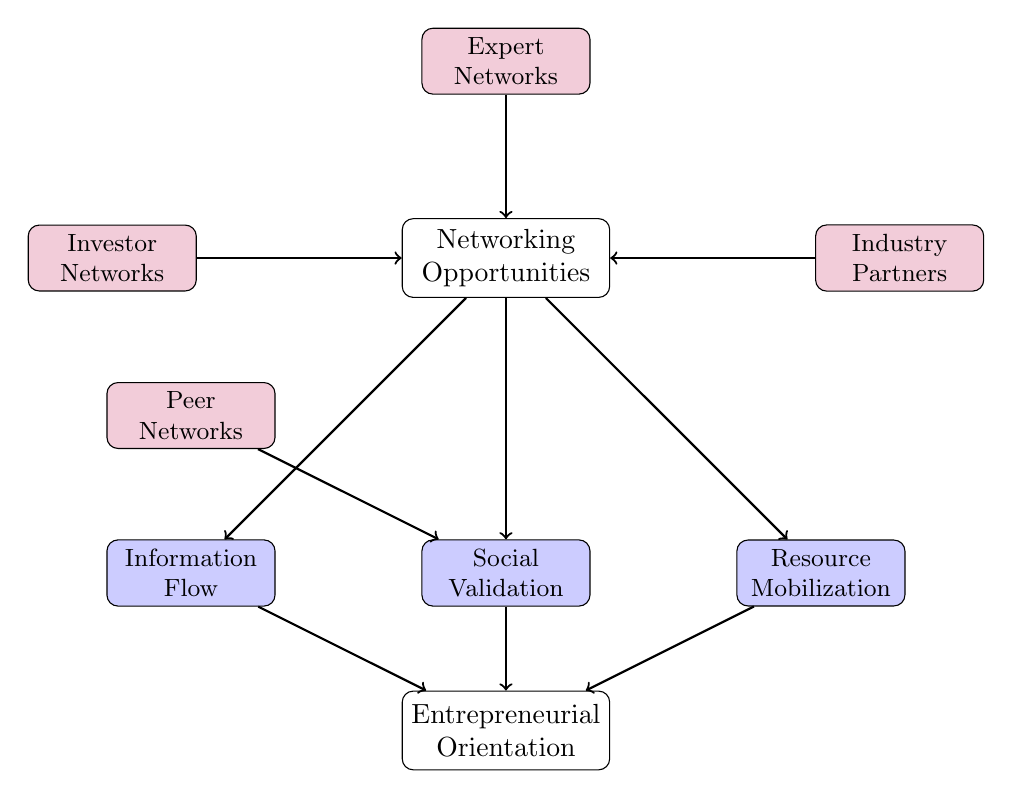
\begin{tikzpicture}[
            box/.style={rectangle, draw, rounded corners, minimum width=2.5cm, minimum height=1cm, text centered, text width=2.4cm},
            arrow/.style={->, thick},
            network/.style={rectangle, draw, rounded corners, fill=purple!20, minimum width=2cm, minimum height=0.8cm, text centered, text width=1.9cm, font=\small},
            benefit/.style={rectangle, draw, rounded corners, fill=blue!20, minimum width=2cm, minimum height=0.8cm, text centered, text width=1.9cm, font=\small}
            ]
            
            % Main variable
            \node[box] (networking) at (0,0) {Networking Opportunities};
            \node[box] (eo) at (0,-6) {Entrepreneurial Orientation};
            
            % Network types
            \node[network] (investors) at (-5,0) {Investor Networks};
            \node[network] (partners) at (5,0) {Industry Partners};
            \node[network] (experts) at (0,2.5) {Expert Networks};
            \node[network] (peers) at (-4,-2) {Peer Networks}; % moved left and down
            
            % Benefits
            \node[benefit] (info) at (-4,-4) {Information Flow};
            \node[benefit] (resources) at (4,-4) {Resource Mobilization};
            \node[benefit] (validation) at (0,-4) {Social Validation};
            
            % Arrows for networks
            \draw[arrow] (investors) -- (networking);
            \draw[arrow] (partners) -- (networking);
            \draw[arrow] (experts) -- (networking);
            \draw[arrow] (peers) -- (validation); % now points to Social Validation
            
            % Arrows for benefits
            \draw[arrow] (networking) -- (info);
            \draw[arrow] (networking) -- (resources);
            \draw[arrow] (networking) -- (validation);
            \draw[arrow] (info) -- (eo);
            \draw[arrow] (resources) -- (eo);
            \draw[arrow] (validation) -- (eo);
            
        \end{tikzpicture}
        \caption{Network Types and Their Contributions to Entrepreneurial Orientation}
        \label{fig:h3_networks}
    \end{figure}

    \subsubsection{Vietnamese Business Culture and Networking}
    The Vietnamese business environment presents unique networking dynamics that enhance the value of UBI-facilitated connections:

    \textbf{Relationship-Oriented Culture}: Strong emphasis on personal relationships and trust in business dealings. 
    \textbf{Fragmented Ecosystem}: Limited natural networking opportunities in the broader entrepreneurial community. 
    \textbf{Trust-Based Transactions}: Business relationships heavily dependent on established trust networks. 
    \textbf{Information Asymmetry}: Limited access to market information and business opportunities.

    \subsubsection{Empirical Evidence}
    Table \ref{tab:h3_evidence} summarizes empirical studies supporting the networking-EO relationship:

    \begin{table}[H]
        \centering
        \caption{Empirical Evidence for H3: Networking Opportunities to Entrepreneurial Orientation}
        \label{tab:h3_evidence}
        \begin{tabular}{|p{3cm}|p{4cm}|p{3cm}|p{2cm}|}
            \hline
            \textbf{Study} & \textbf{Key Finding} & \textbf{Context} & \textbf{Effect Size} \\
            \hline
            \autocite{stam2008entrepreneurial} & Network centrality and diversity positively influence EO & Entrepreneurship & Large \\
            \hline
            \autocite{batjargal2003social} & Social capital enhances entrepreneurial performance & Emerging Markets & Large \\
            \hline
            \autocite{theodorakopoulos2014business} & Networking identified as key success factor in incubation & Business Incubation & Medium \\
            \hline
            \autocite{harper2018makes} & Effective networking distinguishes successful incubators & Incubator Performance & Medium \\
            \hline
        \end{tabular}
    \end{table}

    \subsection{Hypothesis Testing Framework}
    Table \ref{tab:hypothesis_testing} outlines the methodological approach for testing each hypothesis, including the statistical methods, expected outcomes, and practical implications:

    \begin{table}[H]
        \centering
        \caption{Hypothesis Testing Framework and Methodological Approach}
        \label{tab:hypothesis_testing}
        \begin{longtable}{|p{1.5cm}|p{3cm}|p{3cm}|p{3cm}|p{2.5cm}|}
            \hline
            \textbf{Hypothesis} & \textbf{Statistical Test} & \textbf{Expected Result} & \textbf{Measurement Scale} & \textbf{Practical Implication} \\
            \hline
            \endfirsthead
            \multicolumn{5}{c}%
            {\tablename\ \thetable\ -- \textit{Continued from previous page}} \\
            \hline
            \textbf{Hypothesis} & \textbf{Statistical Test} & \textbf{Expected Result} & \textbf{Measurement Scale} & \textbf{Practical Implication} \\
            \hline
            \endhead
            \hline \multicolumn{5}{r}{\textit{Continued on next page}} \\
            \endfoot
            \hline
            \endlastfoot
            
            \textbf{H1} & Multiple Regression & $\beta > 0$, $p < 0.05$ & Likert 1-7 & Enhance mentorship programs \\
            \hline
            \textbf{H2} & Multiple Regression & $\beta > 0$, $p < 0.05$ & Likert 1-7 & Optimize resource allocation \\
            \hline
            \textbf{H3} & Multiple Regression & $\beta > 0$, $p < 0.05$ & Likert 1-7 & Strengthen networking initiatives \\
            \hline
            \textbf{H4} & Multiple Regression & $\beta > 0$, $p < 0.05$ & Likert 1-7 & Focus on EO development \\
            \hline
            \textbf{H5} & Multiple Regression & $\beta > 0$, $p < 0.05$ & Likert 1-7 & Emphasize innovation culture \\
            \hline
            \textbf{H6} & Multiple Regression & $\beta > 0$, $p < 0.05$ & Likert 1-7 & Develop market strategies \\
            \hline
            \textbf{H7} & Multiple Regression & $\beta > 0$, $p < 0.05$ & Likert 1-7 & Prioritize financial planning \\
            \hline
            \textbf{H8} & Multiple Regression & $\beta > 0$, $p < 0.05$ & Likert 1-7 & Direct mentorship impact \\
            \hline
            \textbf{H9} & Multiple Regression & $\beta > 0$, $p < 0.05$ & Likert 1-7 & Resource access benefits \\
            \hline
            \textbf{H10} & Multiple Regression & $\beta > 0$, $p < 0.05$ & Likert 1-7 & Networking value creation \\
            \hline
        \end{longtable}
    \end{table}

    \subsection{Hypothesis 4 (H4): Entrepreneurial Orientation to Startup Performance}
    \textbf{H4: Entrepreneurial Orientation is positively related to startup performance.}

    \subsubsection{Theoretical Foundation}
    \textbf{Strategic Management Theory} \autocite{miller1983correlates, covin1989strategic}: EO as a fundamental strategic orientation driving organizational performance. 
    \textbf{Dynamic Capabilities Theory} \autocite{teece1997dynamic}: EO represents a dynamic capability enabling firms to adapt to changing environments. 
    \textbf{Resource-Based View (RBV)} \autocite{barney1991firm}: EO as a valuable, rare, and inimitable resource creating competitive advantages.

    \subsubsection{Performance Dimensions and EO Impact}
    Figure \ref{fig:h4_performance} illustrates how entrepreneurial orientation influences different dimensions of startup performance:

    \begin{figure}[H]
        \centering
        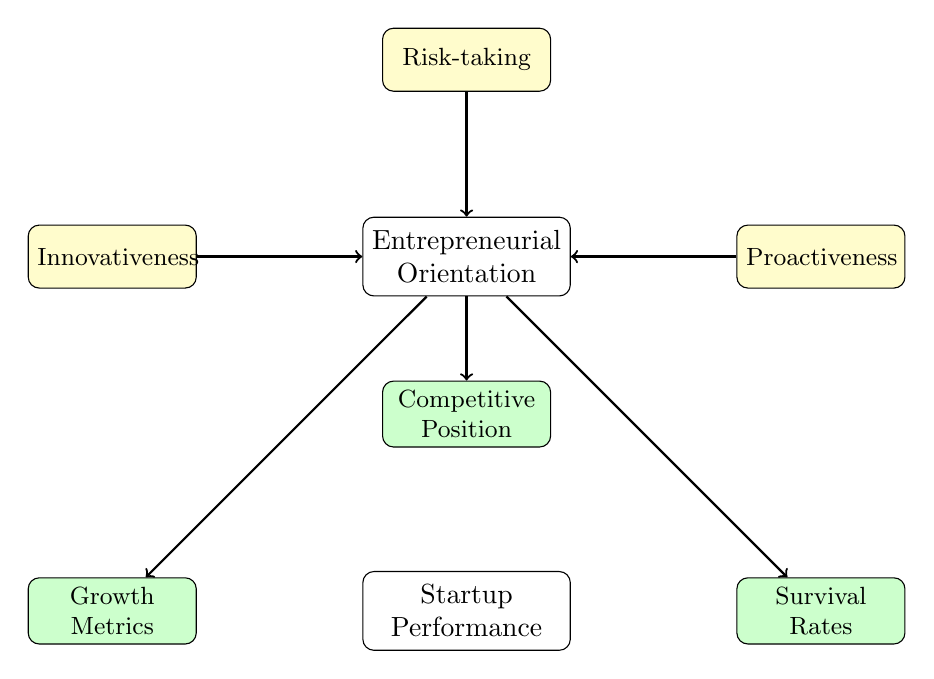
\begin{tikzpicture}[
            node distance=1.5cm,
            box/.style={rectangle, draw, rounded corners, minimum width=2.5cm, minimum height=1cm, text centered, text width=2.4cm},
            arrow/.style={->, thick},
            dimension/.style={rectangle, draw, rounded corners, fill=yellow!20, minimum width=2cm, minimum height=0.8cm, text centered, text width=1.9cm, font=\small},
            outcome/.style={rectangle, draw, rounded corners, fill=green!20, minimum width=2cm, minimum height=0.8cm, text centered, text width=1.9cm, font=\small}
            ]
            
            % Main variable
            \node[box] (eo) {Entrepreneurial Orientation};
            \node[box, below of=eo, yshift=-3cm] (performance) {Startup Performance};
            
            % EO dimensions
            \node[dimension, left of=eo, xshift=-3cm] (innovative) {Innovativeness};
            \node[dimension, right of=eo, xshift=3cm] (proactive) {Proactiveness};
            \node[dimension, above of=eo, yshift=1cm] (risk) {Risk-taking};
            
            % Performance outcomes
            \node[outcome, left of=performance, xshift=-3cm] (growth) {Growth Metrics};
            \node[outcome, right of=performance, xshift=3cm] (survival) {Survival Rates};
            \node[outcome, above of=performance, yshift=1cm] (competitiveness) {Competitive Position};
            
            % Arrows
            \draw[arrow] (innovative) -- (eo);
            \draw[arrow] (proactive) -- (eo);
            \draw[arrow] (risk) -- (eo);
            \draw[arrow] (eo) -- (growth);
            \draw[arrow] (eo) -- (survival);
            \draw[arrow] (eo) -- (competitiveness);
            
        \end{tikzpicture}
        \caption{Entrepreneurial Orientation Dimensions and Performance Outcomes}
        \label{fig:h4_performance}
    \end{figure}

    \subsubsection{Vietnamese Market Context}
    The Vietnamese market environment makes EO particularly critical for startup success:

    \textbf{Rapid Technological Change}: Continuous innovation required to stay competitive. 
    \textbf{International Competition}: Need for proactive market positioning. 
    \textbf{Market Volatility}: Risk-taking essential for capturing opportunities. 
    \textbf{Resource Constraints}: Efficient resource utilization through innovative approaches.

    \subsubsection{Empirical Evidence}
    Table \ref{tab:h4_evidence} presents comprehensive empirical support for the EO-performance relationship:

    \begin{table}[H]
        \centering
        \caption{Empirical Evidence for H4: Entrepreneurial Orientation to Startup Performance}
        \label{tab:h4_evidence}
        \begin{tabular}{|p{3cm}|p{4cm}|p{3cm}|p{2cm}|}
            \hline
            \textbf{Study} & \textbf{Key Finding} & \textbf{Context} & \textbf{Effect Size} \\
            \hline
            \autocite{rauch2009entrepreneurial} & Meta-analysis confirming positive EO-performance relationship & Various Industries & Large \\
            \hline
            \autocite{saeed2014entrepreneurial} & EO particularly beneficial in emerging markets & Emerging Markets & Large \\
            \hline
            \autocite{wales2013entrepreneurial} & Multilevel impact of EO on organizational performance & Multilevel Analysis & Large \\
            \hline
            \autocite{lumpkin1996clarifying} & EO construct clarification and performance linkage & Entrepreneurship & Large \\
            \hline
        \end{tabular}
    \end{table}

    \subsection{Hypothesis 5 (H5): Entrepreneurial Orientation to Innovative Performance}
    The fifth hypothesis asserts that Entrepreneurial Orientation is positively related to innovative performance. Innovation Theory \autocite{schumpeter1934theory}: Entrepreneurial orientation drives innovative outcomes. 
    \textbf{Resource-Based View (RBV)} \autocite{barney1991firm}: Organization's orientation toward innovation is a key driver of innovative outcomes. 
    \textbf{Organizational Learning Theory} \autocite{argyris1978organizational}: EO fosters a learning environment conducive to innovation. The innovativeness component of EO is expected to lead directly to the creation of new products, services, and processes. In Vietnam's rapidly evolving market, where technological change and consumer preferences shift quickly, the ability to innovate continuously is crucial for startup survival and growth \autocite{vietnam_innovation_report_2024}. Empirical research has consistently shown that EO's innovativeness dimension is positively associated with various innovation outcomes, including new product development and process innovation \autocite{lumpkin1996clarifying, wiklund2003knowledge}.

    \subsection{Hypothesis 6 (H6): Entrepreneurial Orientation to Market Performance}
    The sixth hypothesis posits that Entrepreneurial Orientation is positively related to market performance. This assertion is grounded in Market Orientation Theory \autocite{narver1990effect} and the competitive strategy literature \autocite{porter1980competitive}, which suggest that proactive and aggressive market strategies lead to superior market performance. First-Mover Advantage Theory \autocite{lieberman1988first} further posits that early market entry provides competitive advantages. The proactiveness and risk-taking components of EO are expected to drive startups to enter markets early and launch aggressive marketing campaigns, thereby increasing market share and customer acquisition. In Vietnam's competitive market environment, where market share is fiercely contested and customer loyalty is difficult to establish, the ability to proactively identify opportunities and take calculated risks in market development is essential for startup success \autocite{vietnam_innovation_report_2024}. Empirical studies have demonstrated that EO's proactiveness and risk-taking dimensions are positively associated with market performance indicators such as market share growth and customer acquisition \autocite{lumpkin2001linking, wiklund2005entrepreneurial}.

    \subsection{Hypothesis 7 (H7): Entrepreneurial Orientation to Financial Performance}
    The seventh hypothesis asserts that Entrepreneurial Orientation is positively related to financial performance. Strategic Management Theory \autocite{porter1980competitive} and the RBV \autocite{barney1991firm} suggest that strategic orientations that create competitive advantages lead to superior financial performance, while Dynamic Capabilities Theory \autocite{teece1997dynamic} posits that EO enables firms to adapt to changing environments and achieve financial success. Innovative and proactive strategies are expected to lead to new revenue streams and optimized operations, directly improving financial metrics such as revenue and profitability. In Vietnam's challenging business environment, where access to capital is limited and profitability pressures are high, the ability to generate sustainable financial returns through innovative and proactive strategies is crucial for startup survival and growth \autocite{vietnam_innovation_report_2024}. Empirical research has demonstrated that EO is positively associated with various financial performance indicators, including revenue growth and profitability \autocite{rauch2009entrepreneurial, saeed2014entrepreneurial}, with particular benefits observed in emerging markets \autocite{wales2013entrepreneurial}.

    \subsection{Hypothesis 8 (H8): Mentorship Quality to Startup Performance}
    The eighth hypothesis posits that mentorship quality is positively related to startup performance. Human Capital Theory \autocite{becker1964human} asserts that knowledge and expertise are critical resources that directly enhance organizational performance, while Social Capital Theory \autocite{coleman1988social} suggests that mentor relationships provide access to valuable information and resources that improve business outcomes. Timely and strategic advice from a mentor can help a startup avoid costly mistakes and make better business decisions, directly improving its performance across all dimensions. In Vietnam's challenging business environment, where many founders lack experience and the business landscape is complex and rapidly changing, direct mentor guidance is particularly valuable \autocite{dinh2017promoting}. Empirical research has demonstrated that mentorship quality is directly associated with startup performance indicators, including survival rates and revenue growth \autocite{stjean2012mentoring}, with significant improvements observed in emerging markets \autocite{sullivan2011effectiveness}.

    \subsection{Hypothesis 9 (H9): Resource Access to Startup Performance}
    The ninth hypothesis asserts that resource access is positively related to startup performance. The RBV theory \autocite{barney1991firm} emphasizes that access to valuable, rare, and inimitable resources directly creates competitive advantages and superior performance, while Resource Dependency Theory \autocite{pfeffer1978external} suggests that organizational performance is directly influenced by access to critical resources. Access to capital and facilities directly enables a startup to produce, operate, and scale, leading to better business outcomes through immediate operational improvements and strategic opportunities. In Vietnam, where access to capital and technology remains a major barrier for most startups \autocite{vietnam_innovation_report_2024}, direct access to these resources through UBIs can provide immediate and significant performance advantages. Empirical research has consistently shown that resource availability is directly associated with startup performance, including survival rates and growth \autocite{cooper1994initial}, with particular benefits observed in emerging markets \autocite{bruton2010governance}.

    \subsection{Hypothesis 10 (H10): Networking Opportunities to Startup Performance}

    \subsubsection{Theoretical Foundation}
    This hypothesis is grounded in network and social capital theories:

    \begin{itemize}
        \item \textbf{Social Network Theory} \autocite{granovetter1973strength}: Organization's position within networks provides direct access to valuable resources and opportunities
        \item \textbf{Social Capital Theory} \autocite{coleman1988social}: Network relationships create value through information sharing and resource mobilization
        \item \textbf{Resource-Based View (RBV)} \autocite{barney1991firm}: Networks as relational resources that create competitive advantages
    \end{itemize}

    \subsubsection{Direct Performance Impact Mechanisms}
    Figure \ref{fig:h10_mechanisms} illustrates the direct mechanisms through which networking opportunities enhance startup performance:

    \begin{figure}[H]
        \centering
        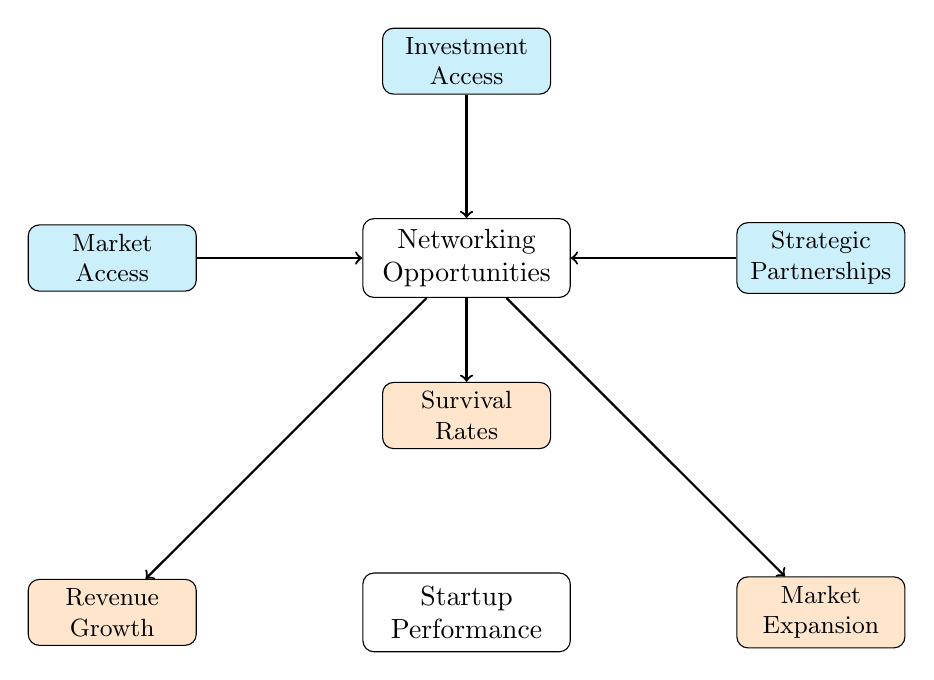
\begin{tikzpicture}[
            node distance=1.5cm,
            box/.style={rectangle, draw, rounded corners, minimum width=2.5cm, minimum height=1cm, text centered, text width=2.4cm},
            arrow/.style={->, thick},
            mechanism/.style={rectangle, draw, rounded corners, fill=cyan!20, minimum width=2cm, minimum height=0.8cm, text centered, text width=1.9cm, font=\small},
            outcome/.style={rectangle, draw, rounded corners, fill=orange!20, minimum width=2cm, minimum height=0.8cm, text centered, text width=1.9cm, font=\small}
            ]
            
            % Main variable
            \node[box] (networking) {Networking Opportunities};
            \node[box, below of=networking, yshift=-3cm] (performance) {Startup Performance};
            
            % Mechanisms
            \node[mechanism, left of=networking, xshift=-3cm] (access) {Market Access};
            \node[mechanism, right of=networking, xshift=3cm] (partnerships) {Strategic Partnerships};
            \node[mechanism, above of=networking, yshift=1cm] (investment) {Investment Access};
            
            % Outcomes
            \node[outcome, left of=performance, xshift=-3cm] (revenue) {Revenue Growth};
            \node[outcome, right of=performance, xshift=3cm] (expansion) {Market Expansion};
            \node[outcome, above of=performance, yshift=1cm] (survival) {Survival Rates};
            
            % Arrows
            \draw[arrow] (access) -- (networking);
            \draw[arrow] (partnerships) -- (networking);
            \draw[arrow] (investment) -- (networking);
            \draw[arrow] (networking) -- (revenue);
            \draw[arrow] (networking) -- (expansion);
            \draw[arrow] (networking) -- (survival);
            
        \end{tikzpicture}
        \caption{Direct Mechanisms Linking Networking Opportunities to Startup Performance}
        \label{fig:h10_mechanisms}
    \end{figure}

    \subsubsection{Vietnamese Business Environment Context}
    The Vietnamese business environment is characterized by a strong relationship-based business culture. In this context, personal connections are not just advantageous but often crucial for achieving business success. Entrepreneurs and startups frequently rely on their networks of acquaintances, friends, and family to access opportunities, resources, and support that might otherwise be unavailable through formal channels.

    Trust networks play a pivotal role in shaping business relationships in Vietnam. The foundation of many business dealings is built on established trust, which is developed over time through repeated interactions and mutual understanding. This reliance on trust means that new entrants to the market may face challenges in building credibility and forming partnerships unless they can demonstrate reliability and integrity within these networks.

    Another defining feature of the Vietnamese business landscape is the prevalence of market information asymmetry. Access to accurate and timely market intelligence is often limited, making it difficult for startups to make informed decisions. As a result, entrepreneurs must frequently depend on informal sources and personal contacts to gather essential information about market trends, customer preferences, and competitive dynamics.

    Finally, resource concentration is a significant factor influencing startup performance in Vietnam. Key resources, such as funding, distribution channels, and strategic partnerships, are often controlled by established networks. This concentration of resources within certain groups or organizations can create barriers to entry for new ventures, underscoring the importance of networking and relationship-building as essential strategies for overcoming these challenges.

    \subsubsection{Empirical Evidence}
    Table \ref{tab:h10_evidence} summarizes empirical studies supporting the direct networking-performance relationship:

    \begin{table}[H]
        \centering
        \caption{Empirical Evidence for H10: Networking Opportunities to Startup Performance}
        \label{tab:h10_evidence}
        \begin{tabular}{|p{3cm}|p{4cm}|p{3cm}|p{2cm}|}
            \hline
            \textbf{Study} & \textbf{Key Finding} & \textbf{Context} & \textbf{Effect Size} \\
            \hline
            \autocite{stam2008entrepreneurial} & Network centrality directly associated with performance & Entrepreneurship & Large \\
            \hline
            \autocite{batjargal2003social} & Social capital enhances performance in emerging markets & Emerging Markets & Large \\
            \hline
            \autocite{spigel2017relational} & Relational aspects significantly influence startup performance & Ecosystem Theory & Medium \\
            \hline
            \autocite{theodorakopoulos2014business} & Networking identified as key success factor & Business Incubation & Medium \\
            \hline
        \end{tabular}
    \end{table}

    \section{Comprehensive Hypothesis Framework}
    Figure \ref{fig:comprehensive_hypothesis_framework} provides a visual synthesis of all ten hypotheses, showing the integrated relationships between UBI support mechanisms, entrepreneurial orientation, and startup performance dimensions:

    \begin{figure}[H]
        \centering
        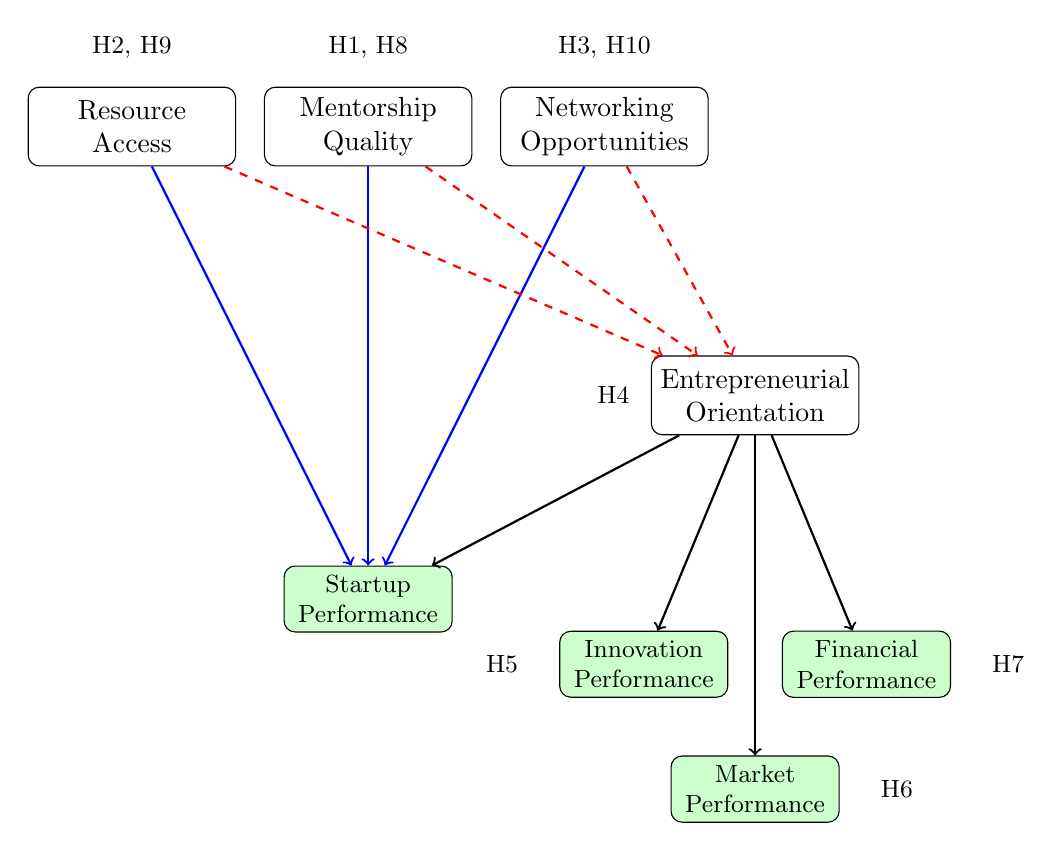
\begin{tikzpicture}[
            node distance=2cm,
            box/.style={rectangle, draw, rounded corners, minimum width=2.5cm, minimum height=1cm, text centered, text width=2.4cm},
            arrow/.style={->, thick},
            direct/.style={->, thick, blue},
            indirect/.style={->, thick, red, dashed},
            performance/.style={rectangle, draw, rounded corners, fill=green!20, minimum width=2cm, minimum height=0.8cm, text centered, text width=1.9cm, font=\small}
            ]
            
            % Independent variables
            \node[box] (mentorship) {Mentorship Quality};
            \node[box, left of=mentorship, xshift=-1cm] (resources) {Resource Access};
            \node[box, right of=mentorship, xshift=1cm] (networking) {Networking Opportunities};
            
            % Mediating variable
            \node[box, below right of=networking, yshift=-2cm, xshift=0.5cm] (eo) {Entrepreneurial Orientation};
            
            % Performance variables
            \node[performance, below of=mentorship, yshift=-4cm] (overall) {Startup Performance};
            \node[performance, below left of=eo, yshift=-2cm] (innovation) {Innovation Performance};
            \node[performance, below right of=eo, yshift=-2cm] (financial) {Financial Performance};
            \node[performance, below of=eo, yshift=-3cm] (market) {Market Performance};
            
            % Direct effects (H8-H10)
            \draw[direct] (mentorship) -- (overall);
            \draw[direct] (resources) -- (overall);
            \draw[direct] (networking) -- (overall);
            
            % Indirect effects through EO (H1-H3)
            \draw[indirect] (mentorship) -- (eo);
            \draw[indirect] (resources) -- (eo);
            \draw[indirect] (networking) -- (eo);
            
            % EO to performance (H4-H7)
            \draw[arrow] (eo) -- (overall);
            \draw[arrow] (eo) -- (innovation);
            \draw[arrow] (eo) -- (financial);
            \draw[arrow] (eo) -- (market);
            
            % Labels
            \node[above of=mentorship, yshift=-1cm] {\small H1, H8};
            \node[above of=resources, yshift=-1cm] {\small H2, H9};
            \node[above of=networking, yshift=-1cm] {\small H3, H10};
            \node[left of=eo, xshift=0.2cm] {\small H4};
            \node[left of=innovation, xshift=0.2cm] {\small H5};
            \node[right of=market, xshift=-0.2cm] {\small H6};
            \node[right of=financial, xshift=-0.2cm] {\small H7};
            
        \end{tikzpicture}
        \caption{Comprehensive Hypothesis Framework}
        \label{fig:comprehensive_hypothesis_framework}
    \end{figure}

    \subsection{Research Implications and Contributions}
    This comprehensive hypothesis framework makes several important contributions to the literature on university-based incubation and startup development:

    \textbf{Theoretical Integration}: Combines multiple theoretical perspectives to explain complex UBI-startup relationships. 
    \textbf{Mediation Analysis}: Examines both direct and indirect effects of UBI support on startup performance. 
    \textbf{Contextual Relevance}: Specifically addresses the Vietnamese entrepreneurial ecosystem. 
    \textbf{Performance Multiplicity}: Considers multiple dimensions of startup performance. 
    \textbf{Practical Applicability}: Provides actionable insights for UBI program optimization.

    The framework provides a robust foundation for empirical testing and offers valuable insights for both academic research and practical UBI management in Vietnam's developing entrepreneurial ecosystem.

\end{document}